\chapter{من النية إلى الحركة}\label{ch:g12:brain-and-movement}

تستيقظ امرأة ذات صباح فلا تستطيع تحريك ذراعها اليمنى ولا ساقها، مع أنها
تحس بهما، وركبتها اليمنى تركل أقوى من أي وقت مضى حين يطرقها الطبيب.
ويبين التصوير رقعة ميتة صغيرة في النصف الأيسر من دماغها، قرب القمة.
وكل ما تحتها سليم --- الأعصاب، والنخاع الشوكي، والأقواس المنعكسة في
الفصل الماضي، والعضلات --- ومع ذلك لا تبلغها نية الحركة. وبعد ستة أشهر
من إعادة التأهيل تمشي، ويبين تصوير دماغها العامل مناطق تضيء لم تكن
تأمر ساقها من قبل. ويتابع هذا الفصل حركة إرادية من القشرة إلى \omterm{def:g12:stretch-reflex:neuron}{العصبون}
الحركي، ويبين كيف ترسم الخريطة التي تأمر بها، وكيف تتقاطع، وكيف يعاد
رسمها.

\section{القشرة الحركية}

\begin{definition}[القشرة الحركية]\label{def:g12:brain-and-movement:cortex}
\emph{القشرة الحركية الأولية}\index{قشرة حركية} شريط من قشرة المخ يمتد
فوق قمة كل نصف كرة، أمام الأخدود الذي يفصل الفص الجبهي عن الجداري
مباشرة. وعصبوناتها منشأ الحركة الإرادية: فمحاويرها تنزل عبر جذع الدماغ
والنخاع الشوكي إلى \omterm{def:g12:stretch-reflex:neuron}{العصبونات} الحركية للعضلات. والشريط \emph{خريطة}
للجسم: فكل جزء منه يأمر جزءًا من الجسم، بترتيب يمتد من القدم عند قمة
نصف الكرة إلى الوجه عند جانبها، ومساحة كل جزء تتناسب لا مع حجم جزء
الجسم بل مع دقة حركاته --- فاليد والوجه يشغلان معظمها.
\end{definition}

\begin{proposition}[الخريطة حقيقية ومتقاطعة]\label{prop:g12:brain-and-movement:map}
تنبيه نقطة من \omterm{def:g12:brain-and-movement:cortex}{القشرة الحركية} كهربائيًا ينتج حركة في جزء الجسم الموافق
في الجانب \emph{المقابل} من الجسم؛ وتضرر نقطة يبطل الحركة الإرادية
لذلك الجزء في الجانب المقابل.
\end{proposition}
\begin{proof}[شواهد]
أثناء جراحة دماغ بتخدير موضعي، طبّق بنفيلد (في ثلاثينيات القرن العشرين)
تيارًا ضعيفًا على نقاط من القشرة المكشوفة وسجل أي العضلات تحركت: فكوّنت
النقاط الخريطة، ومساحتا اليد والوجه خارجتان عن التناسب مع حجمهما، وكل
حركة في الجانب المقابل لنصف الكرة المنبَّه. والتصوير الوظيفي لمتطوعين
أصحاء يحركون إصبعًا واحدة يبدي بقعة نشاط في الموضع المتنبَّأ به في نصف
الكرة المقابل؛ وعند تحريك القدم، بقعة عند القمة. والسكتات التي تخرب
جزءًا من \omterm{def:g12:brain-and-movement:cortex}{قشرة حركية} واحدة تشل الأجزاء المرسومة في الجانب الآخر، مع بقاء
الإحساس.
\end{proof}

\begin{omfigure}
\begin{tikzpicture}
  \node[anchor=south west, inner sep=0] (img) at (0,0)
    {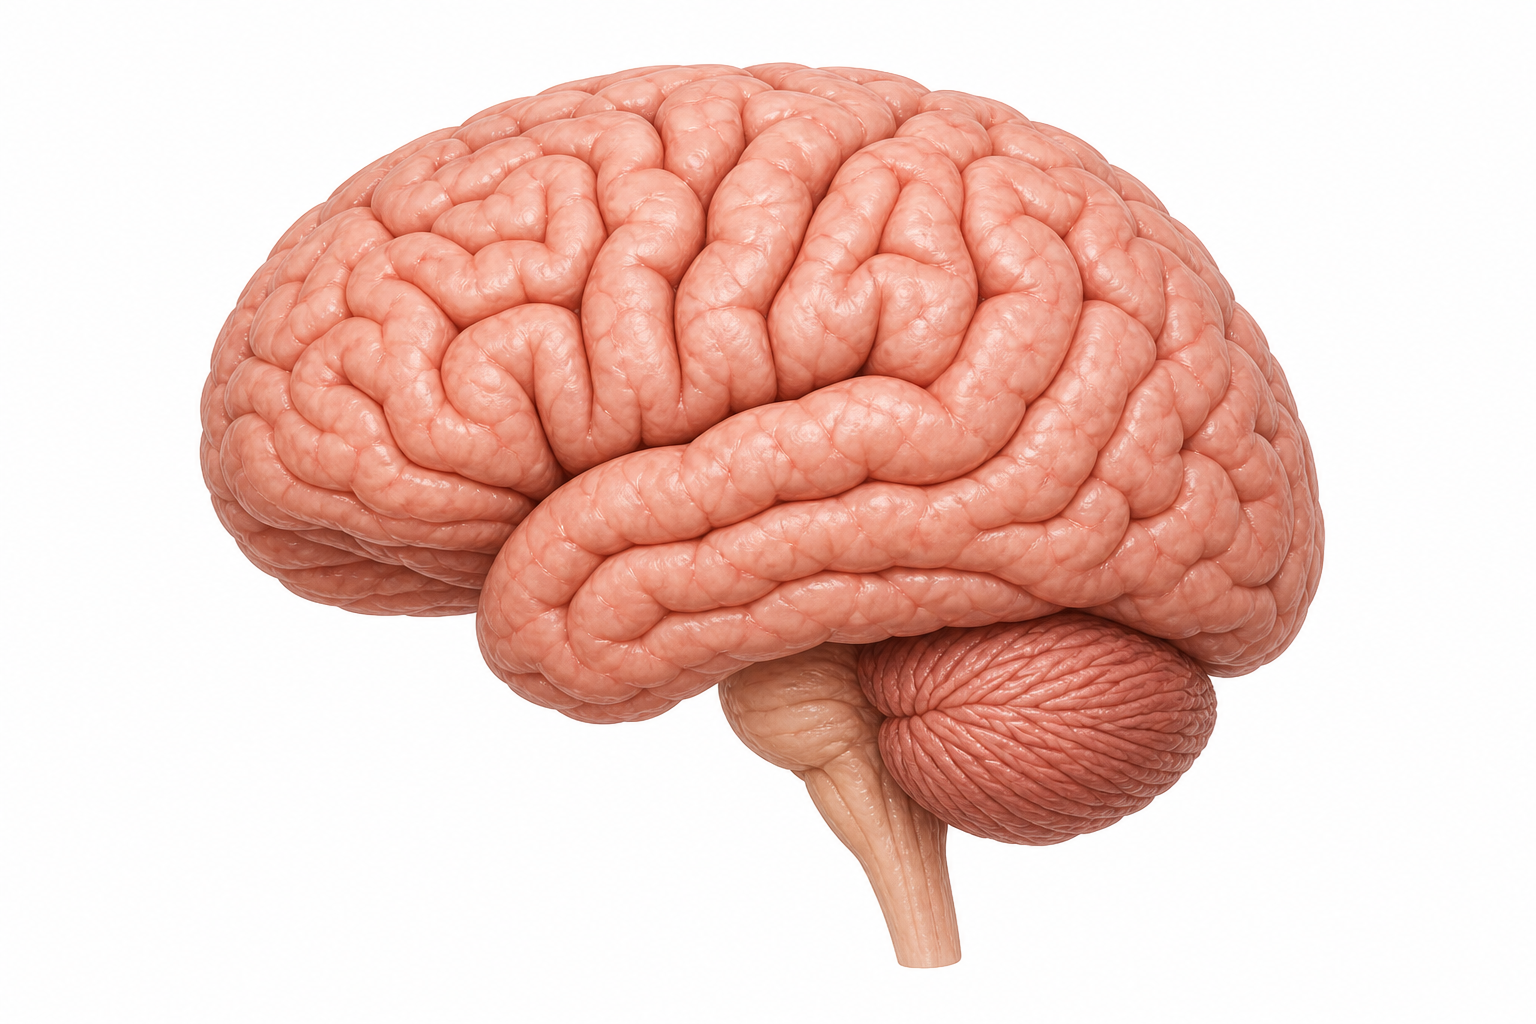
\includegraphics[width=0.52\linewidth]{images/book2/ai/fig-brain-side.png}};
  \begin{scope}[x={(img.south east)}, y={(img.north west)},
      every node/.style={font=\small}]
    \draw[omThm, very thick] (0.50,0.90) .. controls (0.53,0.75) .. (0.58,0.55);
    \draw[omDef, thick] (0.52,0.82) -- (0.45,1.08) node[above, align=center] {القشرة الحركية الأولية\\ (شريط أمام الأخدود المركزي)};
    \draw[omDef, thick] (0.28,0.72) -- (0.10,1.02) node[above] {الفص الجبهي: التخطيط};
    \draw[omDef, thick] (0.72,0.72) -- (0.85,1.02) node[above] {الفص الجداري: الإحساس};
    \draw[omDef, thick] (0.70,0.28) -- (1.04,0.20) node[right] {المخيخ};
    \draw[omDef, thick] (0.60,0.10) -- (0.60,-0.06) node[below] {جذع الدماغ: هنا يتقاطع السبيل};
  \end{scope}
\end{tikzpicture}

{\small الدماغ من اليسار، \omterm{def:g12:brain-and-movement:cortex}{والقشرة الحركية الأولية} معلَّمة بالأحمر:
شريط فوق قمة نصف الكرة، يأمر الجانب الأيمن من الجسم. وألياف النزول
عنده تتقاطع إلى الجانب الآخر في جذع الدماغ.}
\end{omfigure}

\begin{omfigure}
\begin{tikzpicture}
\begin{axis}[
  xbar, bar width=9pt,
  width=0.8\linewidth, height=6cm,
  axis x line=bottom, axis y line=left,
  xmin=0, xmax=35, xlabel={حصة القشرة الحركية (\%)},
  xlabel style={font=\small, at={(axis description cs:0.5,-0.1)}, anchor=north},
  symbolic y coords={الأصابع والقدم, الساق, الجذع, الذراع, اليد والأصابع, الوجه واللسان},
  ytick=data, tick label style={font=\small},
  enlarge y limits=0.12, xtick={0,10,20,30},
  nodes near coords, nodes near coords style={font=\scriptsize, anchor=west},
]
\addplot[fill=omThm!50, draw=omThm] coordinates
  {(4,الأصابع والقدم) (8,الساق) (6,الجذع) (14,الذراع) (32,اليد والأصابع) (30,الوجه واللسان)};
\end{axis}
\end{tikzpicture}

{\small الحصة التقريبية من \omterm{def:g12:brain-and-movement:cortex}{القشرة الحركية} المخصصة لكل جزء من الجسم.
فاليد والوجه، وهما يصنعان أدق الحركات، يأخذان نحو الثلثين؛ والجذع، وهو
يصنع قليلًا منها، يأخذ العشرين. فالمساحة تتبع الدقة، لا الحجم.}
\end{omfigure}

\begin{omfigure}
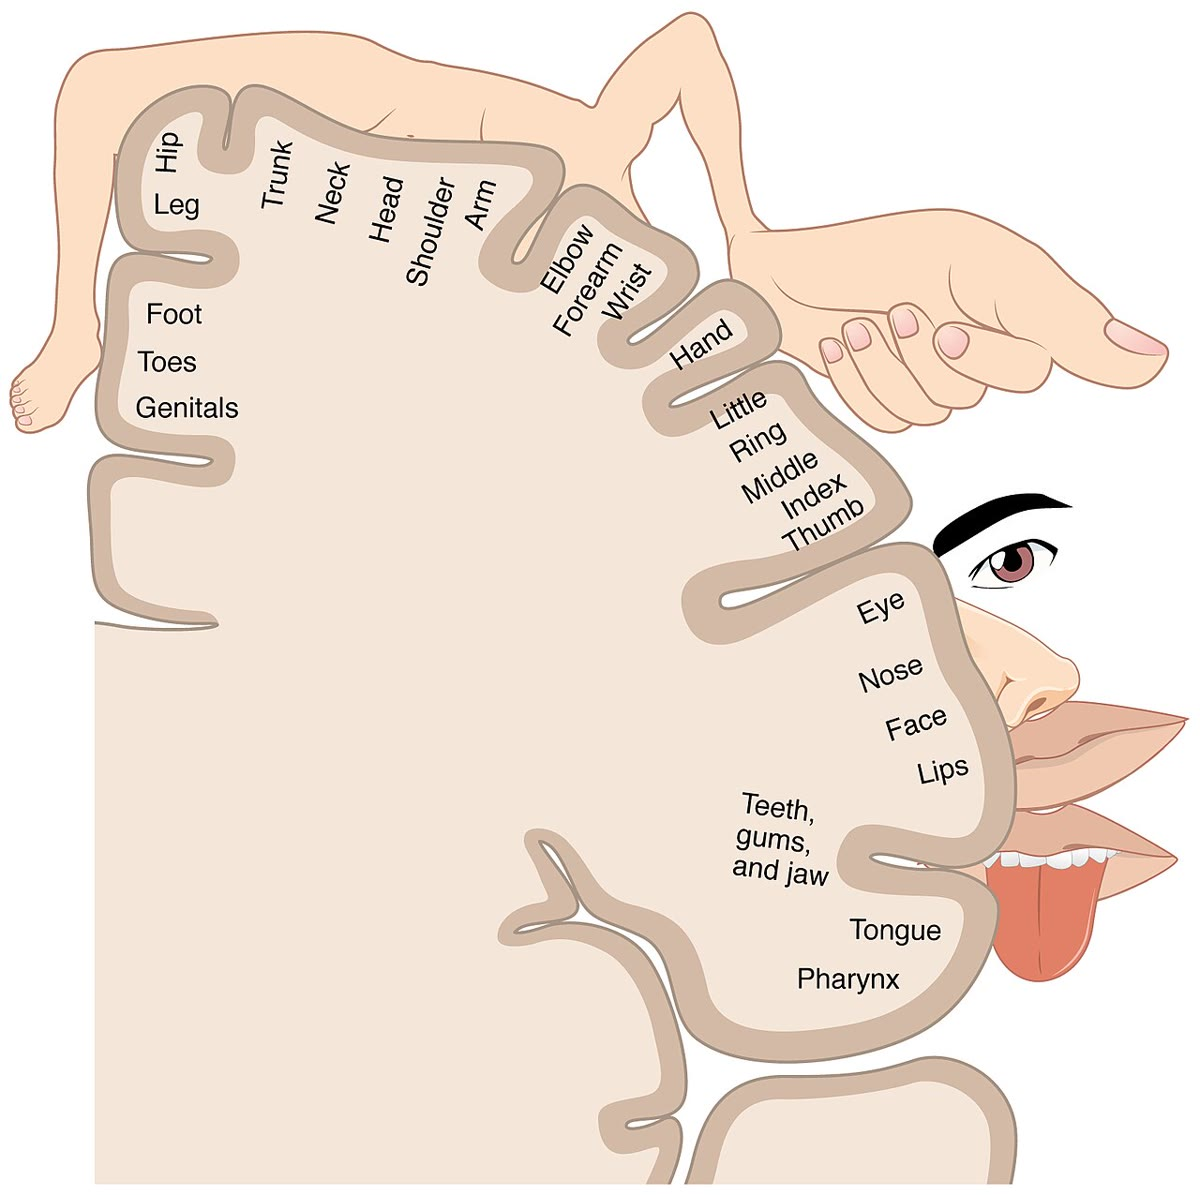
\includegraphics[width=0.5\linewidth]{images/book2/homunculus.jpg}

{\small الخريطة مرسومة جسدًا: كل جزء بحجم القشرة التي يشغلها، موضوعًا فوق مقطع من نصف الكرة. وهذا هو الشريط الحسي، خلف الحركي مباشرة؛ وللخريطة الحركية الترتيب نفسه والنسب نفسها تقريبًا --- فاليد والوجه هائلان، والجذع والساق صغيران. رسم من OpenStax \emph{Anatomy and Physiology}، برخصة CC~BY~3.0.}
\end{omfigure}

\section{السبيل النازل}

\begin{proposition}[من القشرة إلى العصبون الحركي]\label{prop:g12:brain-and-movement:pathway}
محاوير \omterm{def:g12:stretch-reflex:neuron}{عصبونات} \omterm{def:g12:brain-and-movement:cortex}{القشرة الحركية} تؤلف \emph{السبيل القشري
النخاعي}\index{سبيل قشري نخاعي}. وهو ينزل عبر جذع الدماغ، حيث تتقاطع
معظم أليافه إلى الجانب الآخر --- ولهذا كان كل نصف كرة يأمر النصف
المقابل من الجسم --- ويتابع نزولًا في النخاع الشوكي، حيث تغادره عند كل
مستوى ألياف تنتهي على \omterm{def:g12:stretch-reflex:neuron}{العصبونات} الحركية لعضلات ذلك المستوى، أو على
\omterm{def:g12:stretch-reflex:neuron}{عصبونات} بينية إلى جانبها. \omterm{def:g12:stretch-reflex:neuron}{فالعصبون} الحركي في
\cref{ch:g12:stretch-reflex} هو إذن ملتقى أمرين: أمر \omterm{def:g12:stretch-reflex:reflex}{القوس المنعكسة}،
الآتي من المغزل العضلي، وأمر القشرة، الآتي من على بعد متر فوقه.
\end{proposition}
\begin{proof}[شواهد]
تتبع الألياف من القشرة عبر جذع الدماغ يبين التقاطع؛ وآفة في السبيل فوق
التقاطع تشل الجانب المقابل، وتحته تشل الجانب نفسه. وآفة في النخاع
الشوكي تشل كل ما دون مستواها في الجانبين مع بقاء الوجه، إذ تغادر
ألياف الوجه فوقه؛ \omterm{def:g12:stretch-reflex:reflex}{والمنعكسات} دون الآفة تبقى، إذ أقواسها سليمة، وتصير
مبالغًا فيها، إذ لم يعد أثر القشرة المخمِّد يبلغها.
\end{proof}

\begin{omfigure}
\begin{tikzpicture}[font=\small, >=Stealth, line cap=round]
  % left hemisphere box, brainstem, cord, muscles
  \draw[thick, fill=omDef!8, rounded corners=10pt] (-3.4,4.2) rectangle (-0.2,5.8);
  \node at (-1.8,5.0) {القشرة الحركية اليسرى};
  \draw[thick, fill=omDef!8, rounded corners=10pt] (0.2,4.2) rectangle (3.4,5.8);
  \node at (1.8,5.0) {القشرة الحركية اليمنى};
  \draw[thick, fill=gray!15] (-0.8,1.6) rectangle (0.8,3.6);
  \node[font=\scriptsize, anchor=east] at (-0.9,3.3) {جذع الدماغ};
  \draw[thick, fill=gray!10] (-0.6,-2.4) rectangle (0.6,1.6);
  \node[font=\scriptsize, rotate=90] at (0,-0.4) {النخاع الشوكي};
  % tracts: left cortex -> crosses -> right side of cord -> right muscles
  \draw[very thick, omThm] (-1.8,4.2) -- (-0.4,3.4) -- (-0.4,2.6) -- (0.35,2.0) -- (0.35,-1.6);
  \draw[very thick, omDef] (1.8,4.2) -- (0.4,3.4) -- (0.4,2.6) -- (-0.35,2.0) -- (-0.35,-1.6);
  \node[font=\scriptsize, anchor=west] at (0.9,2.3) {التقاطع};
  % motor neurons and muscles
  \fill[omThm] (0.35,-1.6) circle (2.5pt); \draw[very thick, omThm] (0.35,-1.6) -- (2.6,-1.6);
  \draw[thick, fill=omThm!25, rounded corners=5pt] (2.6,-2.0) rectangle (3.8,-1.2); \node[font=\scriptsize] at (3.2,-1.6) {الساق اليمنى};
  \fill[omDef] (-0.35,-1.6) circle (2.5pt); \draw[very thick, omDef] (-0.35,-1.6) -- (-2.6,-1.6);
  \draw[thick, fill=omDef!25, rounded corners=5pt] (-3.8,-2.0) rectangle (-2.6,-1.2); \node[font=\scriptsize] at (-3.2,-1.6) {الساق اليسرى};
  \node[font=\scriptsize, anchor=west, align=left] at (0.9,0.3) {العصبون الحركي: ملتقى\\ أمر القشرة\\ والقوس المنعكسة};
  \draw[gray, thin] (0.9,-0.2) -- (0.5,-1.45);
  \draw[->, thick, gray] (3.2,-2.4) .. controls (2.0,-3.0) and (0.8,-2.6) .. (0.5,-1.8);
  \node[font=\scriptsize, gray, anchor=north] at (2.2,-2.8) {مغزل الساق اليمنى (دخل المنعكس)};
\end{tikzpicture}

{\small \omterm{prop:g12:brain-and-movement:pathway}{السبيل القشري النخاعي}. ألياف من \omterm{def:g12:brain-and-movement:cortex}{القشرة الحركية} اليسرى
(بالأحمر) تتقاطع في جذع الدماغ وتنزل في الجانب الأيمن من النخاع إلى
\omterm{def:g12:stretch-reflex:neuron}{العصبونات} الحركية للساق اليمنى؛ والقشرة اليمنى (بالأزرق) تأمر اليسرى.
وكل \omterm{def:g12:stretch-reflex:neuron}{عصبون} حركي يتلقى أيضًا دخل \omterm{def:g12:stretch-reflex:reflex}{منعكس} عضلته هو.}
\end{omfigure}

\begin{example}[قراءة شلل]\label{ex:g12:brain-and-movement:paralysis}
ذراع وساق يمنيان مشلولان، والوجه كذلك، والإحساس باق: أي آفة في \omterm{def:g12:brain-and-movement:cortex}{القشرة
الحركية} لنصف الكرة الأيسر أو في أليافها فوق التقاطع --- وهي حالة
المرأة في مطلع الفصل. والساقان مشلولتان والذراعان والوجه سليمة،
\omterm{def:g12:stretch-reflex:reflex}{ومنعكسات} الساقين مبالغ فيها: أي النخاع الشوكي متضرر عند مستوى أسفل
الظهر. وذراع واحدة مشلولة رخوة، ومنعكساتها غائبة: أي العصب أو
\omterm{def:g12:stretch-reflex:neuron}{العصبونات} الحركية نفسها، ولا يستطيع شيء دونها أن يطلق. فالخريطة
والتقاطع والقوس تحدد موضع الضرر قبل أي تصوير.
\end{example}

\section{العصبون الحركي يقرر}

\begin{proposition}[التكامل عند العصبون الحركي]\label{prop:g12:brain-and-movement:integration}
\omterm{def:g12:stretch-reflex:neuron}{العصبون} الحركي يتلقى آلاف \omterm{def:g12:stretch-reflex:synapse}{المشابك}: منبِّهة من القشرة ومن المغازل،
ومثبِّطة من \omterm{def:g12:stretch-reflex:neuron}{عصبونات} بينية تقودها مغازل العضلة المضادة، وتقودها القشرة،
وتقودها مراكز أخرى. وكل إشارة واصلة تزيح كمون \omterm{def:g12:stretch-reflex:neuron}{العصبون} قليلًا، نحو
العتبة أو بعيدًا عنها؛ والإزاحات \emph{تتجامع} عبر الميلي ثوان وعبر سطح
\omterm{def:g10:cells-common-unit:cell}{الخلية}، ولا يطلق \omterm{def:g12:stretch-reflex:neuron}{العصبون} إلا حين يعبر مجموعها العتبة. \omterm{def:g12:stretch-reflex:neuron}{فالعصبون} الحركي
ليس إذن مُرحِّلًا بل حاسبة: فالعضلة تتقلص حين تقول ذلك حصيلة كل الأوامر
البالغة عصبوناتها الحركية --- وهو \emph{السبيل النهائي
المشترك}\index{سبيل نهائي مشترك} للحركة.
\end{proposition}
\begin{proof}[شواهد]
التسجيل داخل \omterm{def:g12:stretch-reflex:neuron}{عصبون} حركي يبين كل دخل منبِّه ينتج زوال استقطاب صغيرًا قدره
ميلي فولط أو نحوه، أي أدنى بكثير من \qty{15}{mV} اللازمة؛ ودفقة من
الدخلات، أو دخلات من عدة مصادر دفعة واحدة، متجامعةً إلى العتبة، تنتج
\omterm{prop:g12:stretch-reflex:actionpotential}{كمون عمل}؛ ودخل مثبِّط يصل في اللحظة نفسها يلغي دخلًا منبِّهًا. وقوة
التقلص الإرادي ترتفع بعدد \omterm{def:g12:stretch-reflex:neuron}{العصبونات} الحركية المستقدَمة وبمعدل إطلاقها،
والركلة الركبية أقوى حين يقبض الشخص قبضته --- إذ يضاف تنبيه القشرة إلى
تنبيه المغزل.
\end{proof}

\begin{omfigure}
\begin{tikzpicture}
\begin{axis}[
  width=0.9\linewidth, height=5.6cm,
  axis x line=bottom, axis y line=left,
  xmin=0, xmax=40, ymin=-80, ymax=40,
  xlabel={الزمن (ms)}, ylabel={كمون العصبون الحركي (mV)},
  xlabel style={font=\small, at={(axis description cs:0.5,-0.12)}, anchor=north},
  ylabel style={font=\small},
  tick label style={font=\small}, xtick={0,10,20,30,40}, ytick={-70,-55,0,30},
  clip=false,
]
\addplot[thick, omDef] coordinates {(0,-70) (5,-70) (5.5,-66) (8,-68) (10,-70) (14,-70) (14.5,-66) (16,-64) (17,-61) (18.5,-58) (19.5,-55) (20,-30) (20.5,30) (21,0) (21.5,-50) (22,-75) (25,-72) (28,-70) (30,-70) (30.5,-66) (31.5,-70) (32,-74) (34,-70) (40,-70)};
\draw[dashed, gray] (axis cs:0,-55) -- (axis cs:40,-55);
\node[font=\scriptsize, gray, anchor=south west] at (axis cs:0.3,-55) {العتبة};
\node[font=\scriptsize, anchor=south] at (axis cs:9,-67.5) {دخل منبِّه واحد};
\node[font=\scriptsize, anchor=south, align=center] at (axis cs:11.5,-45) {أربعة دخلات متتابعة\\ سريعًا: المجموع يبلغ العتبة};
\node[font=\scriptsize, anchor=south, align=center] at (axis cs:31,-58) {منبِّه ومثبِّط:\\ يلغي أحدهما الآخر};
\end{axis}
\end{tikzpicture}

{\small التكامل عند \omterm{def:g12:stretch-reflex:neuron}{عصبون} حركي. الدخل المنبِّه الواحد يزيل استقطابه بضعة
ميلي فولط ثم يخبو؛ وعدة دخلات تصل في غضون ميلي ثوان تتجامع إلى العتبة
فيطلق \omterm{def:g12:stretch-reflex:neuron}{العصبون}؛ ودخل مثبِّط يصل مع دخل منبِّه يلغيه.}
\end{omfigure}

\begin{example}[إمساك كأس]\label{ex:g12:brain-and-movement:glass}
عند رفع كأس ملأى، ترسل القشرة تنبيهًا ثابتًا إلى \omterm{def:g12:stretch-reflex:neuron}{العصبونات} الحركية
للذراع؛ وتضيف المغازل تنبيهها وهي تشدّ إذ تميل الكأس؛ وتطرح \omterm{def:g12:stretch-reflex:neuron}{عصبونات}
العضلات المضادة البينية حين تفرط الحركة؛ ويصحح المخيخ، إذ يقارن الحركة
المقصودة بالواقعة، أمر القشرة بعد عشرات الميلي ثوان. وكل \omterm{def:g12:stretch-reflex:neuron}{عصبون} حركي
يجمع المحادثة كلها ويطلق بالقدر الكافي لا غير. وسلاسة الحركة هي توازن
تلك المجاميع.
\end{example}

\section{خريطة يمكن أن يعاد رسمها}

\begin{proposition}[لدونة القشرة الحركية]\label{prop:g12:brain-and-movement:plasticity}
الخريطة الحركية ليست ثابتة. فتمرين حركة يوسّع المساحة القشرية التي
تأمر بها ويشحذ وصلاتها؛ ومساحة طرف تنكمش حين يشل الطرف عن الحركة،
وتستولي عليها الأجزاء المجاورة بعد بتر. وبعد سكتة، تستطيع القشرة
السليمة حول الآفة، والمساحة الموافقة في نصف الكرة الآخر، أن تتعلم أمر
العضلات المصابة --- شرط أن تستعمل: فإعادة التأهيل تعمل بإكراه الحركة،
مرارًا، حتى تنتقى الدارات الناجية وتقوى. ولدونة \cref{ch:g11:vision-and-brain}
تنطبق على جانب الدماغ الآمر كما تنطبق على جانبه الحاس.
\end{proposition}
\begin{proof}[شواهد]
تصوير قشرة عازفي الكمان يبدي مساحة موسَّعة لأصابع اليد اليسرى، بنسبة
العمر الذي بدأوا فيه؛ وبعد خمسة أيام من تمرين تتابع بالأصابع، يبدي
متطوعون عاديون مساحة موسَّعة قابلة للقياس لتلك الأصابع، تنكمش ثانية إذا
توقف التمرين. وبعد السكتة، المرضى الذين تدرَّب ذراعهم المشلولة تدريبًا
مكثفًا --- مع تقييد الذراع السليمة --- يستعيدون وظيفة أكثر مما يستعيد
من يعوّضون بالذراع السليمة، ويبين التصوير أن الحركة المستعادة تأمر بها
مناطق مجاورة للآفة. والقردة التي تصاب مساحة أصابعها بآفة لا تستعيد
حركة الأصابع إلا إذا مرّنت الأصابع.
\end{proof}

\begin{omfigure}
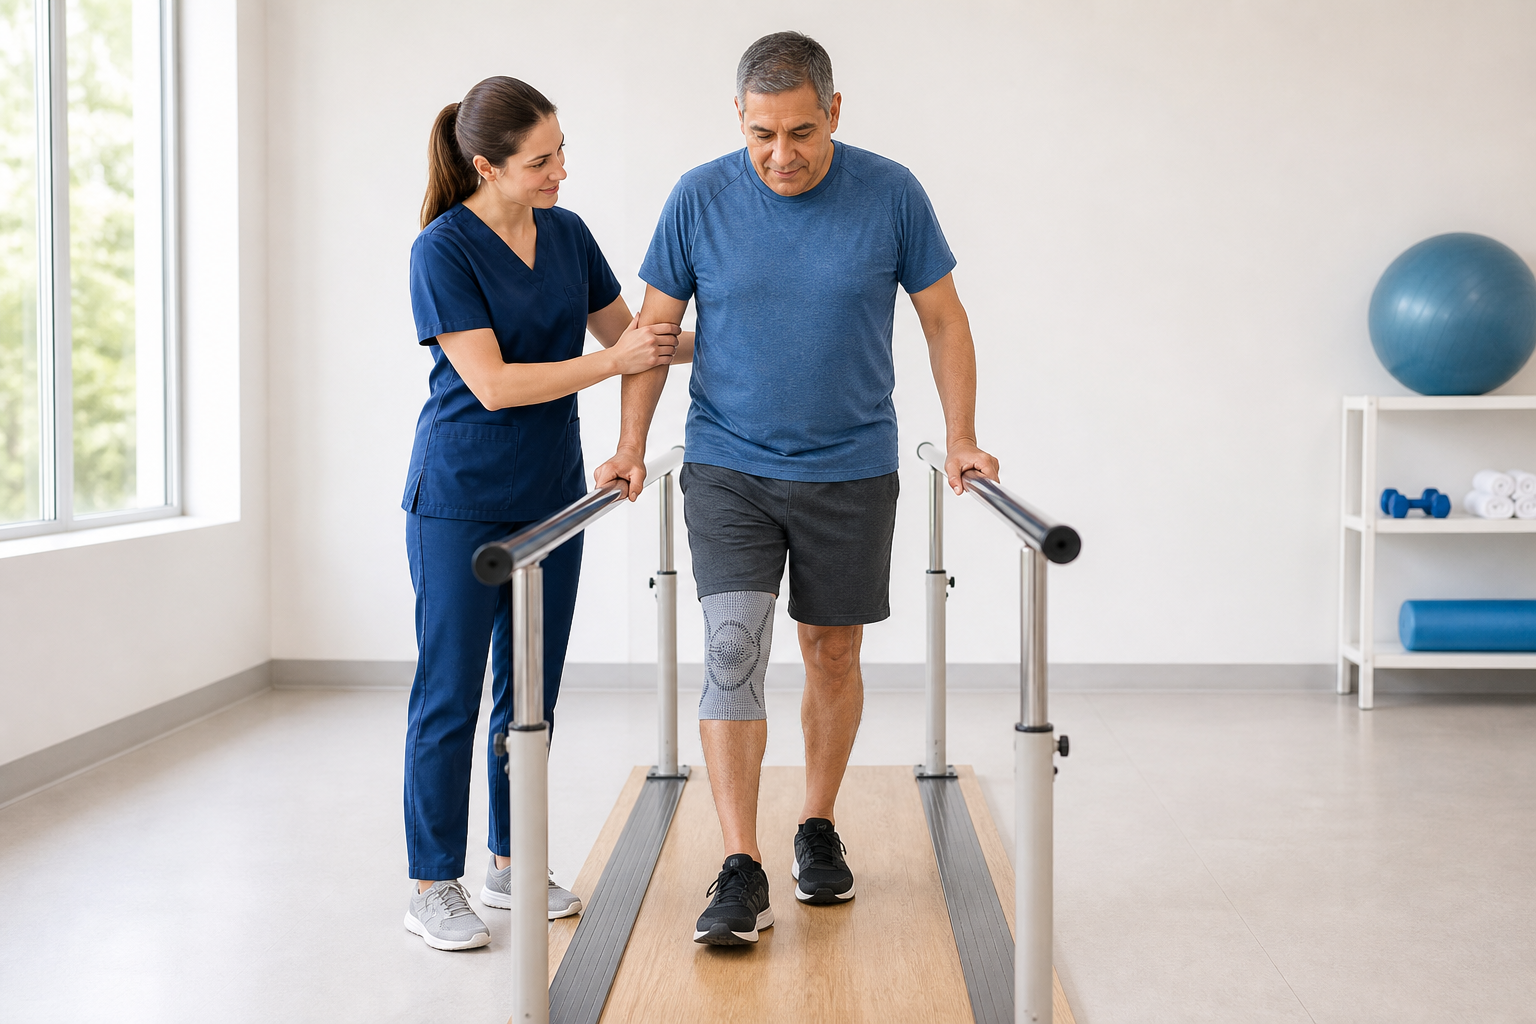
\includegraphics[width=0.56\linewidth]{images/book2/ai/g12-move-rehab.png}

{\small إعادة التأهيل بعد سكتة: إعادة تعلم المشي بين قضيبين متوازيين.
فكل خطوة مكرَهة تنتقي الدارات الناجية القادرة على أمر الساق وتقويها،
ويعاد رسم الخريطة القشرية حول الآفة.}
\end{omfigure}

\begin{example}[ستة أشهر بعد السكتة]\label{ex:g12:brain-and-movement:sixmonths}
الأسبوع 1: الساق اليمنى لا تتحرك؛ ومنعكساتها مبالغ فيها. والأسابيع من
2 إلى 6: المعالج الفيزيائي يحرك الساق، ثم يجعل المريضة تحاول كل حركة؛
فيعود تقلص خافت. والأشهر من 2 إلى 4: مشي بين القضيبين، ألف خطوة في
اليوم؛ ويبين التصوير نشاطًا ينتشر في القشرة حول الآفة وفي نصف الكرة
الآخر. والشهر 6: مشي بعكاز. والآفة لم تلتئم --- \omterm{def:g12:stretch-reflex:neuron}{فعصبونات} القشرة لا
تعود نموًا --- لكن دارات مجاورة استقدمت، وكل خطوة من خطوات التعافي
صنعت بمحاولة الحركة.
\end{example}

\begin{method}[تحديد موضع اضطراب حركي]\label{met:g12:brain-and-movement:locate}
\begin{enumerate}
  \item أي الأجزاء مصاب؟ جانب واحد من الجسم والوجه معه: أي نصف الكرة
        المقابل أو أليافه فوق التقاطع. وجانبان دون مستوى، والوجه سليم:
        أي النخاع الشوكي عند ذلك المستوى. وطرف واحد أو مجموعة عضلات لا
        غير: أي عصبها أو عصبوناتها الحركية.
  \item أالمنعكسات محفوظة؟ مبالغ فيها: أي القوس سليمة والإخماد القشري
        مفقود (فالآفة فوق \omterm{def:g12:stretch-reflex:neuron}{العصبون} الحركي). وغائبة: أي القوس نفسها
        مقطوعة (\omterm{def:g12:stretch-reflex:neuron}{فالعصبون} الحركي أو العصب أو العضلة).
  \item أالإحساس محفوظ؟ فالعجز الحركي الخالص يدل على السبيل الحركي؛
        والمختلط على آفة تصيب الاثنين.
  \item ما الذي يمكن أن يستعاد؟ آفات القشرة، باللدونة \omterm{def:g10:sport-and-health:training}{والتدريب}؛ ونخاع
        أو عصب مقطوع، أقل بكثير؛ وأمراض العضلة \omterm{def:g12:stretch-reflex:neuron}{والعصبون} الحركي، بحسب
        سببها.
\end{enumerate}
\end{method}

\begin{remark}[حلقة السنة الأخيرة]\label{rem:g12:brain-and-movement:loop}
نية الحركة نمط من \omterm{prop:g12:stretch-reflex:actionpotential}{كمونات العمل} في شريط من القشرة؛ ينزل مترًا من
المحوار، ويتقاطع، ويزنه \omterm{def:g12:stretch-reflex:neuron}{عصبون} حركي في مقابل \omterm{def:g12:stretch-reflex:reflex}{منعكس} العضلة التي سيحركها؛
وتتقلص العضلة بانزلاق الخييطات، مدفوعَ الثمن من \omterm{def:g12:respiration-fermentation:atp}{ATP} \omterm{def:g10:cells-common-unit:organelle}{المتقدرات}، على
غلوكوز حرره الكبد تحت عين البنكرياس، وعلى أكسجين سلّمه القلب
والرئتان --- والقشرة التي أعطت الأمر شكّلها استعمالها هي خريطةً كما هي.
وكل فصل من فصول هذا الكتاب كان قطعة من تلك الحلقة. والمجلدات التالية
تفتح كل قطعة أكثر؛ ولا واحد منها يغير الحلقة.
\end{remark}

\section{تمارين}

\begin{exercise}[$\star$]\label{exo:g12:brain-and-movement:1}
أين تقع \omterm{def:g12:brain-and-movement:cortex}{القشرة الحركية الأولية}، وماذا تمثل خريطتها؟
\end{exercise}

\begin{exercise}[$\star$]\label{exo:g12:brain-and-movement:2}
صف \omterm{prop:g12:brain-and-movement:pathway}{السبيل القشري النخاعي} من القشرة إلى عضلة في الساق، مسميًا أين
يتقاطع.
\end{exercise}

\begin{exercise}[$\star$]\label{exo:g12:brain-and-movement:3}
لماذا تأخذ اليد من \omterm{def:g12:brain-and-movement:cortex}{القشرة الحركية} أكثر مما يأخذ الجذع كله؟
\end{exercise}

\begin{exercise}[$\star$]\label{exo:g12:brain-and-movement:4}
ماذا يعني "\omterm{prop:g12:brain-and-movement:integration}{السبيل النهائي المشترك}" بالنسبة إلى \omterm{def:g12:stretch-reflex:neuron}{العصبون} الحركي؟
\end{exercise}

\begin{exercise}[$\star$]\label{exo:g12:brain-and-movement:5}
أعط شاهدين على أن الخريطة الحركية يمكن أن تتغير.
\end{exercise}

\begin{exercise}[$\star\star$]\label{exo:g12:brain-and-movement:6}
من شكل التكامل، بكم يزيل الدخل المنبِّه الواحد استقطاب \omterm{def:g12:stretch-reflex:neuron}{العصبون}، وكم
دخلًا يلزم في غضون ميلي ثوان قليلة لبلوغ العتبة، وماذا يحدث حين يتزامن
دخل مثبِّط مع دخل منبِّه؟
\end{exercise}

\begin{exercise}[$\star\star$]\label{exo:g12:brain-and-movement:7}
مريض لا يستطيع تحريك الجانب الأيسر من وجهه ولا ذراعه اليسرى؛ وساقه
اليسرى ضعيفة. حدد موضع الآفة، مستعينًا بالخريطة وبالتقاطع.
\end{exercise}

\begin{exercise}[$\star\star$]\label{exo:g12:brain-and-movement:8}
فسّر لماذا يبالغ في الركلة الركبية بعد سكتة تشل الساق، ولماذا تبطل حين
يقطع العصب الذاهب إلى الساق.
\end{exercise}

\begin{exercise}[$\star\star$]\label{exo:g12:brain-and-movement:9}
شخص قطع نخاعه الشوكي في وسط الظهر: فأي الحركات تفقد، وأي \omterm{def:g12:stretch-reflex:reflex}{المنعكسات}
تبقى، ولماذا لا يصاب الوجه؟
\end{exercise}

\begin{exercise}[$\star\star$]\label{exo:g12:brain-and-movement:10}
فسّر، بالتكامل، لماذا يجعل قبض القبضتين الركلة الركبية أقوى.
\end{exercise}

\begin{exercise}[$\star\star$]\label{exo:g12:brain-and-movement:11}
مساحة أصابع عازفة بيانو أكبر من مساحة غير الموسيقي، وأكبر منها أيضًا
إن كانت قد بدأت قبل السابعة. فسّر الأمرين.
\end{exercise}

\begin{exercise}[$\star\star\star$]\label{exo:g12:brain-and-movement:12}
بعد سكتة، تقييد الذراع السليمة وإكراه استعمال المشلولة يعطي تعافيًا
أفضل من ترك المريض يعوّض. فسّر بانتقاء الدارات، واربط ذلك بهررة
\cref{ch:g11:vision-and-brain}.
\end{exercise}

\begin{exercise}[$\star\star\star$]\label{exo:g12:brain-and-movement:13}
مبتور يحس يده المفقودة حين تلمس وجنته، ويبين التصوير أن مساحة الوجه قد
امتدت إلى مساحة اليد السابقة. فسّر، وقل بم يتنبأ ذلك في \omterm{def:g12:brain-and-movement:cortex}{القشرة الحركية}
في الجانب نفسه.
\end{exercise}

\begin{exercise}[$\star\star\star$]\label{exo:g12:brain-and-movement:14}
مرض يخرب \omterm{def:g12:stretch-reflex:neuron}{العصبونات} الحركية في النخاع الشوكي والقشرة سليمة؛ وآخر يخرب
\omterm{def:g12:brain-and-movement:cortex}{القشرة الحركية} \omterm{def:g12:stretch-reflex:neuron}{والعصبونات} الحركية سليمة. قارن المريضين: الشلل،
\omterm{def:g12:stretch-reflex:reflex}{والمنعكسات}، وضمور العضلات، وما تستطيع واجهة بين الدماغ والآلة أن تفعله
لكل منهما.
\end{exercise}

\begin{exercise}[$\star\star\star$]\label{exo:g12:brain-and-movement:15}
"تعلم حركة تغير في العضلات." صحّح الجملة في فقرة، مستعينًا بالخريطة
القشرية، وبتكامل \omterm{def:g12:stretch-reflex:neuron}{العصبون} الحركي، وباللدونة.
\end{exercise}

\section{مسألة: نصف الكرة الأيسر}

\begin{problem}[{مسألة نهاية الأسبوع --- سكتة تقرأ من الأعراض إلى
الآفة، وحساب العصبون الحركي، والخريطة يعاد رسمها عبر ستة أشهر، وحلقة
السنة كلها تغلق}]
\label{pb:g12:brain-and-movement:1}
امرأة في الثانية والستين تستيقظ وذراعها اليمنى وساقها مشلولتان والجانب
الأيمن من وجهها متدلٍّ؛ والإحساس طبيعي؛ والركلة الركبية اليمنى مبالغ
فيها واليسرى طبيعية. ويبين التصوير آفة قدرها \qty{2}{cm} في الجزء
العلوي من نصف الكرة الأيسر.

\medskip
\noindent\textbf{القسم الأول --- تحديد الموضع.}
\begin{enumerate}
  \item فسّر لماذا كانت الآفة في اليسار مع أن العجز في اليمين.
  \item أي جزء من الخريطة مصاب؟ برهن من أجزاء الجسم الثلاثة المعنية.
  \item ولماذا كان الإحساس طبيعيًا؟ وأي شريط من القشرة سلم؟
  \item ولماذا كانت الركلة الركبية اليمنى مبالغًا فيها لا مبطلة؟
  \item ومريض ثان عنده الشلل نفسه لكن ركلته الركبية غائبة وعضلاته
        ضامرة. حدد موضع آفته وفسّر الفرق.
\end{enumerate}

\medskip
\noindent\textbf{القسم الثاني --- حساب \omterm{def:g12:stretch-reflex:neuron}{العصبون} الحركي.}
\omterm{def:g12:stretch-reflex:neuron}{عصبون} حركي في الساق اليمنى عتبته \qty{15}{mV} فوق كمون راحته. وكل دخل
قشري يزيل استقطابه \qty{1}{mV}، وكل دخل مغزلي \qty{2}{mV}، وكل دخل
مثبِّط من \omterm{def:g12:stretch-reflex:neuron}{عصبون} العضلة المضادة البيني \qty{-2}{mV}؛ والدخلات تتجامع إذا
وصلت في غضون \qty{5}{ms}.
\begin{enumerate}[resume]
  \item قبل السكتة، أرسلت خطوة إرادية 12 دخلًا قشريًا وأرسل المغزل 3 في
        غضون \qty{5}{ms}. أأطلق \omterm{def:g12:stretch-reflex:neuron}{العصبون}؟
  \item وأثناء الخطوة نفسها وصل أيضًا دخلان مثبِّطان. اجمع من جديد.
  \item وبعد السكتة صارت الدخلات القشرية صفرًا. فما المجموع أثناء
        محاولة خطوة؟ وماذا تفعل الساق؟
  \item ويطرق الطبيب الركبة: فيرسل المغزل 10 دخلات في غضون \qty{5}{ms}.
        وقبل السكتة كانت القشرة ترسل أيضًا 3 دخلات مثبِّطة (مخمِّدة)
        أثناء الطرقة؛ وبعدها لا شيء. احسب المجموعين وفسّر المبالغة في
        الركلة.
  \item وبعد ثلاثة أشهر عادت الدخلات القشرية إلى 8 في الخطوة. فمع 3 من
        المغزل، أيطلق \omterm{def:g12:stretch-reflex:neuron}{العصبون}؟ وكيف تتوقع أن تبدو الحركة؟
\end{enumerate}

\medskip
\noindent\textbf{القسم الثالث --- الخريطة معادًا رسمها.}
\begin{enumerate}[resume]
  \item \omterm{def:g12:stretch-reflex:neuron}{عصبونات} الآفة الميتة لا تعود نموًا. فمن أين تستطيع الدخلات
        القشرية في السؤال 10 أن تأتي؟
  \item وإعادة التأهيل تقتضي أن تحاول المريضة الحركة آلاف المرات. فسّر،
        باللدونة، لماذا كانت المحاولة مهمة ولماذا لا يكفي تحريك المعالج
        للساق تحريكًا سلبيًا.
  \item والتصوير في الشهر الرابع يبدي نشاطًا في مساحة الساق في نصف
        الكرة الأيمن أثناء خطوة بالساق اليمنى. فأي الألياف تستطيع أن
        تحمل ذلك الأمر، بالنظر إلى التقاطع؟
  \item ويد المريضة اليمنى تتعافى أقل من ساقها. اقترح تفسيرًا من
        الخريطة ومن متطلبات حركات اليد.
  \item قارن تعافيها بتعافي هرة أعيد فتح عينها المغلقة بعد الطور
        الحرج. ما المشترك، وما المختلف؟
\end{enumerate}

\medskip
\noindent\textbf{القسم الرابع --- الحلقة تغلق.}
\begin{enumerate}[resume]
  \item تتبع خطوة واحدة من مشيتها المستعادة من القشرة إلى التقلص: سمّ
        السبيل، والتقاطع، والملتقى، والناقل عند العضلة، ومصدر \omterm{def:g12:respiration-fermentation:atp}{ATP}
        العضلة.
  \item والخطوة تكلف عضلاتها \omterm{def:g12:respiration-fermentation:atp}{ATP} مصنوعًا من غلوكوز حرره الكبد. سمّ
        \omterm{def:g11:hormones-and-reproduction:hormone}{الهرمون} الذي أتاح للكبد تحريره والعضو الذي قاس الحاجة.
  \item والأكسجين اللازم لذلك \omterm{def:g12:respiration-fermentation:atp}{ATP} سلّمه قلب يخفق أسرع. سمّ الآليتين
        اللتين رفعتا تواتره في بداية المشي.
  \item وتعافيها توقف على اللدونة؛ وسكتتها على شريان مسدود؛ ونجاتها على
        \omterm{def:g12:innate-immunity:immunity}{المناعة الفطرية} والتكيّفية وهما تلقيان عداوى سرير المستشفى. سمّ
        فصلًا واحدًا من هذا المجلد لكل واحد منها.
  \item اذكر النتيجة: الجانب وشريط القشرة حيث تقع الآفة، ومجموع
        الدخلات الذي يجعل عصبونًا حركيًا يطلق، وخاصة القشرة التي أعادت
        إليها ساقها.
\end{enumerate}
\end{problem}
